% Created 2019-12-21 Sat 00:35
\documentclass[a4paper,12pt]{article}
\usepackage[utf8]{inputenc}
\usepackage[T1]{fontenc}
\usepackage{fixltx2e}
\usepackage{graphicx}
\usepackage{longtable}
\usepackage{float}
\usepackage{wrapfig}
\usepackage{rotating}
\usepackage[normalem]{ulem}
\usepackage{amsmath}
\usepackage{textcomp}
\usepackage{marvosym}
\usepackage{wasysym}
\usepackage{amssymb}
\usepackage{hyperref}
\tolerance=1000
\usepackage[margin=3cm]{geometry} 	   % Choose your margin here.
\usepackage{tikz,pgfplots}
\usetikzlibrary{calc,patterns,arrows,decorations.pathmorphing,decorations.markings}
\usetikzlibrary{circuits}
\usepackage{randomwalk}
\usepackage{schemabloc}
\usepackage{blox}
\usepackage{array,makecell,multirow}
\pgfplotsset{width=16cm,height=6cm, compat=1.8}
\usepackage{amsmath,mathtools,amssymb,mathrsfs}
\usetikzlibrary{automata, positioning}
\setcounter{secnumdepth}{3}
\author{nybo}
\date{\today}
\title{main}
\hypersetup{
  pdfkeywords={},
  pdfsubject={},
  pdfcreator={Emacs 25.2.2 (Org mode 8.2.10)}}
\begin{document}

\maketitle
\tableofcontents

\newpage
\section{Randomness}
\label{sec-1}


\subsection{Monte carlo}
\label{sec-1-1}
assume table with 50/50 red black
\subsubsection{Gamblers fallcaly}
\label{sec-1-1-1}
If the soccerteam have won/lost 10 times in a row
 they have loose/win next match. 


\subsubsection{Regession to the mean - Francis Galton, 1885}
\label{sec-1-1-2}
If the parents are taller than the mean will the child 
be shorter than the mean. No bioligy, just analysing the 
data.\\
What is says: after na extreme event, you are likley to
 get an less extreme event. After spinning 10 reds. You 
are likley to get less than 10 reds on your next 
10 spins, but the expected number is still 5. \\
Now if one is looking at the avrage of the 20 
spins it will be closer to the mean, ie. 
regression to the mean. 



\subsubsection{Summed up: why are these different?}
\label{sec-1-1-3}
\begin{enumerate}
\item The gambler fallacy sais that we are expected to have
\end{enumerate}
fewer than 5 reds on the 10 spins. \\ 2. Regression to the mean
 sais that we will probably have fewer than 10 reds on the next. \\
\begin{enumerate}
\item Below the mean. \\ 2. closer to the mean.
\end{enumerate}



\subsection{Sample space}
\label{sec-1-2}
\subsubsection{Girl boy paradox}
\label{sec-1-2-1}
My Friend Nik has two kids, and he told you he has at least one a girl, hence what is the probability of the other kid is female?

\begin{equation*}
\begin{array}{c|c | c}
{\text { First kid }} & {\text { Second Kid }} &P() \\ 
\hline \text { Boy } & {\text { Boy }} &1/4  \\
 {\text { Boy }} & {\text { Girl }}    &1/4  \\ 
{\text { Girl }} & {\text { Girl }}    &1/4  \\ 
{\text { Girl }} & {\text { Boy }}     &1/4
\end{array}
\end{equation*}
You saw my friend Nik was walking on the street with his daughter. And Nik told you he got another child at home, so, what is the probability of the other child was a female?

\subsubsection{Monty Hall problem}
\label{sec-1-2-2}
\begin{table}[h!]
\centering
\begin{tabular}{l |l |l |l}
Behind door 1 & Behind door 2 & Behind door 3 & P() \\
\hline
Goat          & Goat          & Car           & 1/3 \\
Goat          & Car           & Goat          & 1/3 \\
Car           & Goat          & Goat          & 1/3
\end{tabular}
\end{table}


Still not convinced? Take a 100 doors, would you still switch?


\subsection{Random prosesses}
\label{sec-1-3}

\subsubsection{Random walk}
\label{sec-1-3-1}

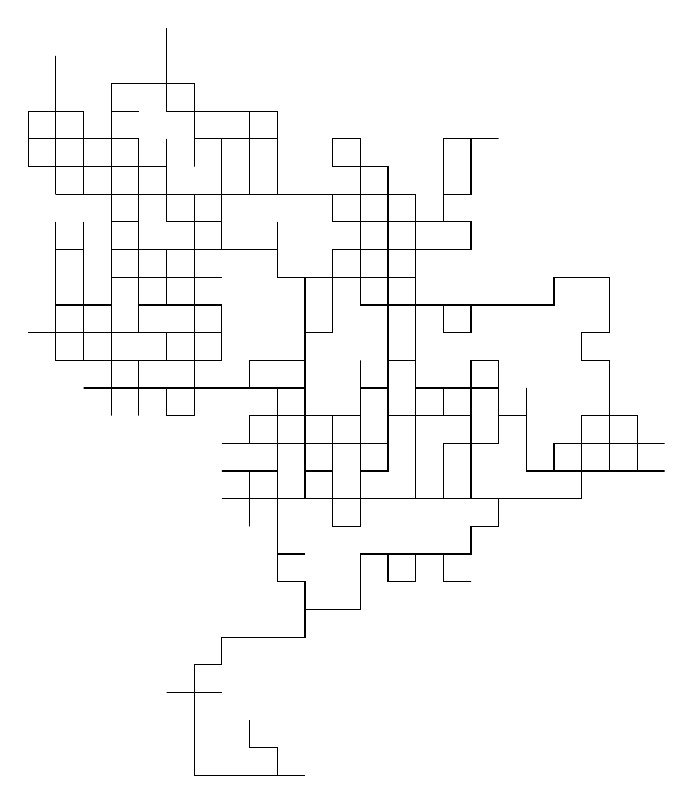
\begin{tikzpicture}
\node[anchor=center,inner sep=0,every picture/.style={draw=red, thick}](randdes)
    {\RandomWalk {number=800, angles = {0, 90, 180, 270}, degrees}};
\end{tikzpicture}

\subsubsection{makrov chian}
\label{sec-1-3-2}
The makrov property/ assumption
$$
 Pr(X_{n+1}=x\mid X_{1}=x_{1},X_{2}=x_{2},\ldots ,X_{n}=x_{n})=\Pr(X_{n+1}=x\mid X_{n}=x_{n})
$$

\begin{equation*}
\begin{aligned} p_{i j} &=\mathbf{P}\left(X_{n+1}=j | X_{n}=i\right) \\ &=\mathbf{P}\left(X_{n+1}=j | X_{n}=i, X_{n-1}, \ldots, X_{0}\right) \end{aligned}
\end{equation*}
 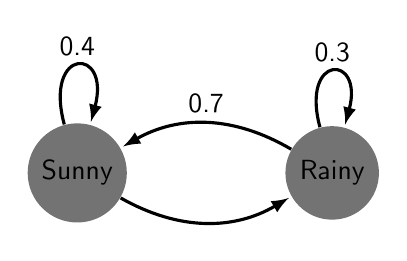
\begin{tikzpicture}[font=\sffamily]

 % Add the states
 \node[state,
       draw=none,
       fill=gray!90!black] (s) {Sunny};
 \node[state,
       right=2cm of s,
       draw=none, 
       fill=gray!90!black] (r) {Rainy};

 % Connect the states with arrows
 \draw[every loop,
       auto=right,
       line width=0.4mm,
       >=latex]
     (s) edge[bend right, auto=left]  node {$$} (r)
     (r) edge[bend right, auto=right] node {0.7} (s)
     (s) edge[loop above]             node {0.4} (s)
     (r) edge[loop above]             node {0.3} (r);
\end{tikzpicture}
$\backslash$


Random walk does not have a transission probility matrix since the state space are not finite.
For markov chian with finite state space matrecies we just have an matrix describing all 
the probabilities.


\section{PDF}
\label{sec-2}
\subsection{Normal distribution}
\label{sec-2-1}
$$
\frac{1}{\sqrt{2 \pi \sigma^{2}}} e^{-\frac{(x-\mu)^{2}}{2 \sigma^{2}}}
$$
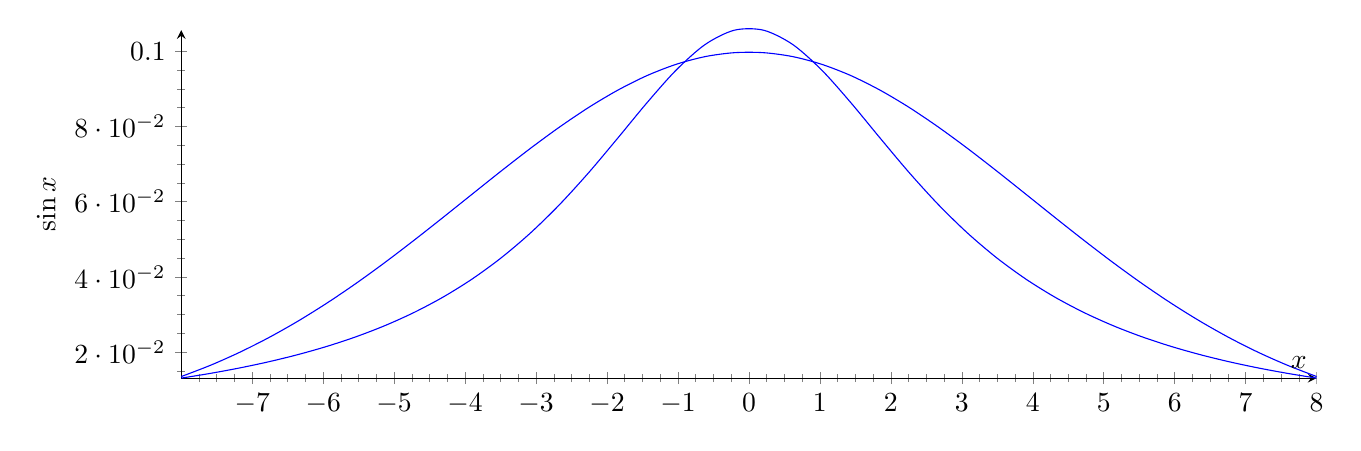
\begin{tikzpicture}
\begin{axis}[
   clip= false,
        minor tick num=3,
        axis y line=left,
        axis x line=middle,
        xlabel=$x$,ylabel=$\sin x$
        ]
        \addplot[smooth,blue,mark=none,
                 domain=-8:8,samples=40] 
                {1/(4*sqrt(2*pi))*exp(-((x-0)^2)/(2*4^2))};
        \addplot[smooth,blue,mark=none,
                 domain=-8:8,samples=40] 
                {1/(pi*3*(1+((x-0)/3)^2))};
\end{axis}
\end{tikzpicture}

\subsection{Cauchy distribution}
\label{sec-2-2}
$$
\frac{1}{\pi \gamma\left[1+\left(\frac{x-x_{0}}{\gamma}\right)^{2}\right]}
$$

\begin{tikzpicture}
\begin{axis}[
        minor tick num=3,
        axis y line=left,
        axis x line=middle,
        xlabel=$x$,ylabel=$\sin x$
        ]
        \addplot[smooth,blue,mark=none,
                 domain=-8:8,samples=40] 
                {1/(pi*5*(1+((x-0)/5)^2))};
\end{axis}
\end{tikzpicture}



\subsection{Together}
\label{sec-2-3}
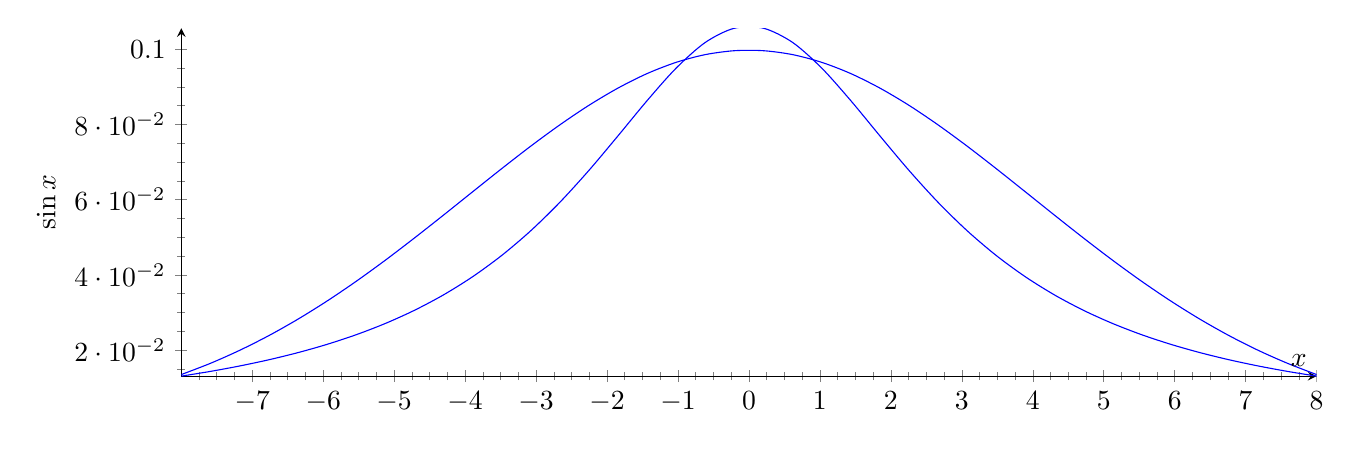
\begin{tikzpicture}
\begin{axis}[
        minor tick num=3,
        axis y line=left,
        axis x line=middle,
        xlabel=$x$,ylabel=$\sin x$
        ]
        \addplot[smooth,blue,mark=none,
                 domain=-8:8,samples=40] 
                {1/(4*sqrt(2*pi))*exp(-((x-0)^2)/(2*4^2))};
        \addplot[smooth,blue,mark=none,
                 domain=-8:8,samples=40] 
                {1/(pi*3*(1+((x-0)/3)^2))};
\end{axis}
\end{tikzpicture}


\section{Learning}
\label{sec-3}

\subsection{supervised vs unsupervised learning}
\label{sec-3-1}


\begin{tikzpicture}
\draw [-latex] (-1,0) -- (5,0) node [above left]  {$x$};
\draw [-latex] (0,-1) -- (0,5) node [below right] {$y$};
\draw[dashed]   (6,3) node[solid, cross out,draw=black] {};
\draw[dashed]   (5,2) node[solid, cross out,draw=black] {};
\draw[dashed]   (5.5,4) node[solid, cross out,draw=black] {};
\draw[dashed]   (5,3) node[solid, cross out,draw=black] {};
\draw[dashed]   (2,3) node[solid, fill=white, circle,draw=black] {};
\draw[dashed]   (2,2) node[solid, fill=white, circle,draw=black] {};
\draw[dashed]   (1.4,2) node[solid, fill=white, circle,draw=black] {};
\draw[dashed]   (1,3) node[solid, fill=white, circle,draw=black] {};
\end{tikzpicture}
\begin{tikzpicture}
\draw [-latex] (-1,0) -- (5,0) node [above left]  {$x$};
\draw [-latex] (0,-1) -- (0,5) node [below right] {$y$};
\draw[dashed]   (6,3) node[solid, cross out,draw=black] {};
\draw[dashed]   (5,2) node[solid, cross out,draw=black] {};
\draw[dashed]   (5.5,4) node[solid, cross out,draw=black] {};
\draw[dashed]   (5,3) node[solid, cross out,draw=black] {};
\draw[dashed]   (2,3) node[solid, cross out,draw=black] {};
\draw[dashed]   (2,2) node[solid, cross out,draw=black] {};
\draw[dashed]   (1.4,2) node[solid, cross out,draw=black] {};
\draw[dashed]   (1,3) node[solid, cross out,draw=black] {};
\end{tikzpicture}


\newpage

\section{Ordbok}
\label{sec-4}
\subsection{Vehicles}
\label{sec-4-1}
RPAS 
AUV 
ROV

\section{Moving average / moving variance}
\label{sec-5}
Digital filter
\begin{equation}
\begin{aligned}
&y(k)=\frac{1}{N+1} \sum_{n=0}^{n} b_{N} u(k-n)\\
&y(k)=b_{0} u(k)+b_{1} u(k-1) \ldots b_{N} u(k-n)
\end{aligned}
\end{equation}


let $n$ be the size of the filter, and $y_k$ be the mesurments
\begin{align*} 
y'_k &=y_{k}\frac{1}{n}+y_{k-1}\frac{1}{n}+y_{k-2}\frac{1}{n}+\dots+y_{k-n+1}\frac{1}{n}\\
     &=\frac{1}{n}\sum_{i=0}^{n-1}y_{k-i} 
\end{align*}


\subsection{analyse of 6}
\label{sec-5-1}
\begin{equation}
\begin{aligned}
&y(k)=\frac{1}{N+1} \sum_{n=0}^{n} u(k-n)\\
&y(k)=\frac{1}{6} \sum_{n=0}^{n} u(k-n)
\end{aligned}
\end{equation}

\begin{equation}
\begin{aligned}
y(k) &=\frac{1}{6}[u(k-n)+u(k-1)+u(k-2)+u(k-3)+u(k-4)+u(k-5)] \\
\mathcal{Z}\{y(k)\} &=\frac{1}{6}\left[z+z^{-1}+z^{-2}+z^{-3}+z^{-4}+z^{-5}\right] \\
Y(z) &=\frac{1}{6} \cdot \frac{1+z^{1}+z^{2}+z^{3}+z^{4}+z^{5}}{z^{5}}
\end{aligned}
\end{equation}


Frekvens respons (demping)
\begin{equation}
\begin{aligned}
&Y(j w)=\frac{1}{6}\left(1+e^{j w T s} \cdots\right)\\
&|Y(w)|=\frac{1}{N}\left|\frac{\sin \left(\frac{w N}{2}\right)}{\sin \left(\frac{w}{2}\right)}\right|
\end{aligned}
\end{equation}


\section{Chaos and Bifurcations}
\label{sec-6}
\subsection{example}
\label{sec-6-1}
$\ddot{x}+0.1 \dot{x}+x^{5}=6 \sin t$
\begin{equation}
\begin{array}{l}{x(0)=2, \quad \dot x(0)=3} \\
 {x(0)=2.01, \quad \dot{x}(0)=3.01}\end{array}
\end{equation}
from x 0 to 50 


\section{to be added}
\label{sec-7}
winer process 
markov process
random walk
% Emacs 25.2.2 (Org mode 8.2.10)
\end{document}